
\section{Features Engineering}\label{sec:features-engineering}
The intrustion detection scheme~\cite{intrustion_detection_using_mouse_dynamics}, while also using the Balabit dataset as it was intended to be used, extracted a set of features from the raw mouse position data.
Though their work implemented a supervised learning-based binary classifier, the features they extracted were proven to be effective metrics in differentiating and identifying users.
Instead of using all 6 elements of a datapoint vector, as outlined in the \textit{Balabit Dataset} section~\ref{subsec:balabit-dataset}, we elected to only use the client timestamp ($t$), x position ($x$), and y position ($y$) values.
These three values construct a triplet, ($t_i$, $x_i$, $y_i$), $i = 1{\dots}n$, where $n$ is the number of recorded mouse positions, or datapoint vectors, in a session file.
The three values, time and 2d coordinates, of a mouse position datapoint are all that is needed to generate the mouse movement features in this thesis research.
From these three values, or triplets, of a single datapoint vector, in the list of vectors of a session file, the following features were extracted:
\begin{itemize}
    \item \textbf{velocity}: $v_i = \frac{\Delta p_i}{\Delta t_i}$, where $\Delta p_i = \lvert p_{i+1} - p_i \rvert$ and $\Delta t_i = t_{i+1} - t_i$
    \item \textbf{horizontal velocity}: ${v_x}_i = \frac{\Delta x_i}{\Delta t_i}$, where $\Delta x_i = \lvert x_{i+1} - x_i \rvert$ and $\Delta t_i = t_{i+1} - t_i$
    \item \textbf{vertical velocity}: ${v_y}_i = \frac{\Delta y_i}{\Delta t_i}$, where $\Delta y_i = \lvert y_{i+1} - y_i \rvert$ and $\Delta t_i = t_{i+1} - t_i$
    \item \textbf{acceleration}: $a_i = \frac{\Delta v_i}{\Delta t_i}$, where $\Delta v_i = \lvert v_{i+1} - v_i \rvert$ and $\Delta t_i = t_{i+1} - t_i$
    \item \textbf{jerk}: $j_i = \frac{\Delta a_i}{\Delta t_i}$, where $\Delta a_i = \lvert a_{i+1} - a_i \rvert$ and $\Delta t_i = t_{i+1} - t_i$
    \item \textbf{theta}: $\Theta _i = \arctan 2(\frac{\Delta y_i}{\Delta x_i})$, where $\Delta y_i = \lvert y_{i+1} - y_i \rvert$ and $\Delta x_i = \lvert x_{i+1} - x_i \rvert$
\end{itemize}

\subsection{Realtime Generation}\label{subsec:realtime-generation}
As described in the objective, this implementation is meant to detect web bots and botnet attacks in realtime.
At this stage of the detection scheme, a program would need to be run in realtime to compute the 6 features outline above.
Initially, a Python program was used to generate these 6 features as described.
The program calculated all 1676 session files, from all 10 users, in an average of 7 minutes.
By pre-allocating lists of numeric values, and incrementing a counter variable that keeps track of where to insert the next calculated feature value into the list of numeric values, the runtime was reduced from 7 minutes to slightly more than 3 minutes.
Further, the entire features generator program was converted from Python to Golang.

\begin{figure}[!h]
    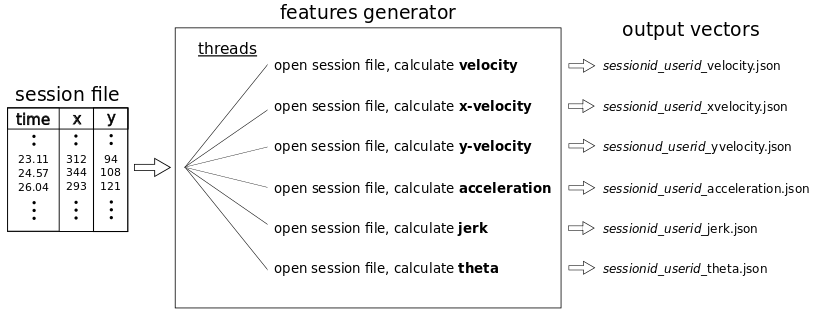
\includegraphics[width=1\columnwidth]{figures/parallelized_features_generator}
    \caption{Parallelization of the features generator}
    \label{fig:parallelization-of-the-features-generator-implementation-version}
    {\small There are 6 Go routines, or threads as shown in this diagram, that parallelize the features generation stage of the system design. Figure~\ref{fig:distribution-of-the-parallelize-features-generator} displays how this parallelized features generator can be distributed.}
\end{figure}

By creating Go-routines on each of the 6 features, the average runtime of the Golang program calculating all 1676 sessions files was less than 30 seconds.
Figure~\ref{fig:parallelization-of-the-features-generator-implementation-version} shows the parallelization of calculating the 6 features.
All runtimes for realtime feature generation do not include data cleaning and prep.
Since the Balabit dataset has many duplicate timestamp values, with different \textit{x} and \textit{y} values, a pre-generation step would need to take place to remove erooneous duplicates, as a means to "clean" the raw data input.

\subsection{Statistics}\label{subsec:statistics}
After the $n$ feature values have been generated, where $n$ is the number of datapoint vectors or triplets in a session, for each of the 6 features, the values would need to be represented with statistical values.
The statistical values used for each of the 6 features are \textbf{mean}, \textbf{median}, \textbf{mode}, \textbf{interquartile range}, \textbf{minimum}, \textbf{maximum}, \textbf{range}, and \textbf{standard deviation}.

It is worth noting that the \textit{mode} and \textit{minimum} values did not appear to be as useful as the other statistical metrics.
The minimum values of each of the feature values lists were mostly zero.
This is a result of the feature calculations.
For example, horizontal velocity could be zero if the $x$ position does not change in two successive datapoint vectors.
Formally, ${v_x}_i = \frac{\Delta x_i}{\Delta t_i} = 0$ if $\Delta x_i = \lvert x_i - x_{i+1} \rvert = 0$, meaning $x_i = x_{i+1}$.
This is one example of why the \textit{maximum} and \textit{range} values were often the same.
If $range = \vert maximum - minimum \rvert$, where $mimimum = 0$, than $range = maxmimum$.

